\documentclass[12pt]{article} % use larger type; default would be 10pt

\usepackage{pgfplots}
\usetikzlibrary{calc}
\usetikzlibrary{arrows}
\usetikzlibrary{patterns}
\usetikzlibrary{calc,intersections,through,backgrounds}
\usetikzlibrary{decorations.pathreplacing}
        \newcommand\degree[0]{^{\circ}}
        \newcommand\abs[1]{\left|#1\right|}

\title{Play with TikZ}
\author{Just Us}
%\date{} % Activate to display a given date or no date (if empty),
         % otherwise the current date is printed 

\begin{document}
\maketitle

\section{10.2 Polar Graphs }




exam10-4-1 vectors 

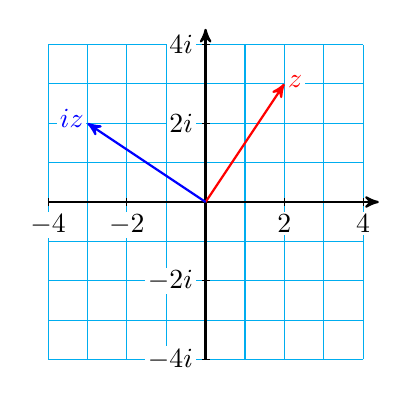
\begin{tikzpicture} [scale=.5]
\draw[cyan] (-4,-4) grid (4,4);
\foreach \y in {-4,-2,2,4} {
\draw[black] (.1,\y) --++ (-.2,0) node[left, xshift=-2, fill=white, inner sep=1]{$\y i$};
}
\foreach \x in {-4,-2,2,4} {
\draw[black] (\x,.1) --++ (0,-.2) node[below, yshift=-2, fill=white, inner sep=1]{$\x$};
}
\coordinate (O) at (0,0);
\coordinate (z) at (2,3);
\coordinate (z2) at (-3,2);
\draw[black,thick,->,>=stealth'] (-4,0)--(4.4,0);
\draw[black,thick,->,>=stealth'] (0,-4)--(0, 4.4);
\draw[red, thick, ->, >=stealth'] (O) -- ++(z) node[above right, yshift=-.1cm, fill=white, inner sep=1]{$z$};
\draw[blue, thick, ->, >=stealth'] (O) -- ++(z2) node[above left, yshift=-.1cm, fill=white, inner sep=1]{$iz$};
\end{tikzpicture}
\newline


exer10-4-1ans vectors 

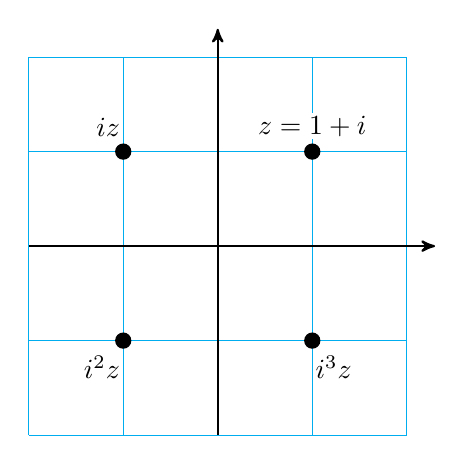
\begin{tikzpicture} [scale=1.2]
\draw[cyan] (-2,-2) grid (2,2);
\coordinate (O) at (0,0);
\coordinate (z) at (1,1);
\coordinate (z2) at (-1,1);
\coordinate (z3) at (-1,-1);
\coordinate (z4) at (1,-1);
\draw[black,thick,->,>=stealth'] (-2,0)--(2.3,0);
\draw[black,thick,->,>=stealth'] (0,-2)--(0, 2.3);
\filldraw[black] (z) circle (.08cm) node[above, yshift=.15cm, fill=white, inner sep=1]{$z=1+i$};
\filldraw[black] (z2) circle (.08cm) node[above left, yshift=.15cm, fill=white, inner sep=1]{$iz$};
\filldraw[black] (z3) circle (.08cm) node[below left, yshift=-.15cm, fill=white, inner sep=1]{$i^2 z$};
\filldraw[black] (z4) circle (.08cm) node[below right, yshift=-.15cm, fill=white, inner sep=1]{$i^3 z$};
\end{tikzpicture}
\newline


fig10-4-1 polar form of complex number 

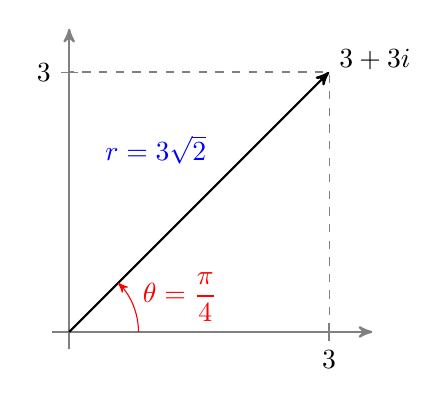
\begin{tikzpicture} [scale=1.1]
\coordinate (O) at (0,0);
\coordinate (z) at (3,3);
\coordinate (z2) at (3,0);
\coordinate (z3) at (0,3);
\draw[gray,thick,->,>=stealth'] (-.2,0)--(3.5,0);
\draw[gray,thick,->,>=stealth'] (0,-.2)--(0, 3.5);
\draw[gray,dashed] (z2)--(z)--(z3);
\draw[gray] (3,.1) --++ (0,-.2) node[below, text=black] {$3$}; 
\draw[gray] (.1,3) --++ (-.2,0) node[left, text=black] {$3$}; 
\draw[black,thick,->,>=stealth'] (O) -- (z) node[above right, yshift=-.1cm] {$3+3i$}; 
\draw[red, ->,>=stealth'] (0:0.8) arc (0:45:0.8) node[right, yshift=3, midway] {$\theta =\displaystyle\frac{\pi}{4}$};
\node[blue] at (1,2.1) {$r=3\sqrt{2}$};
\end{tikzpicture}
\newline


exam10-4-2 polar form of complex number 

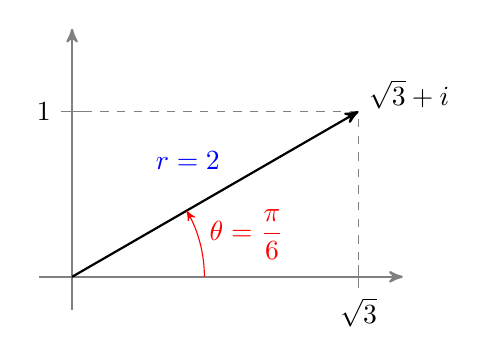
\begin{tikzpicture} [scale=2.1]
\coordinate (O) at (0,0);
\coordinate (z) at (30:2);
\coordinate (z2) at ({sqrt(3)},0);
\coordinate (z3) at (0,1);
\draw[gray,thick,->,>=stealth'] (-.2,0)--(2,0);
\draw[gray,thick,->,>=stealth'] (0,-.2)--(0, 1.5);
\draw[gray,dashed] (z2)--(z)--(z3);
\draw[gray] ({sqrt(3)},.07) --++ (0,-.14) node[below, text=black] {$\sqrt{3}$}; 
\draw[gray] (.07,1) --++ (-.14,0) node[left, text=black] {$1$}; 
\draw[black,thick,->,>=stealth'] (O) -- (z) node[above right, yshift=-.1cm] {$\sqrt{3}+i$}; 
\draw[red, ->,>=stealth'] (0:0.8) arc (0:30:0.8) node[right, yshift=3, midway] {$\theta =\displaystyle\frac{\pi}{6}$};
\node[blue] at (0.7,0.7) {$r=2$};
\end{tikzpicture}
\newline



exam10-4-3

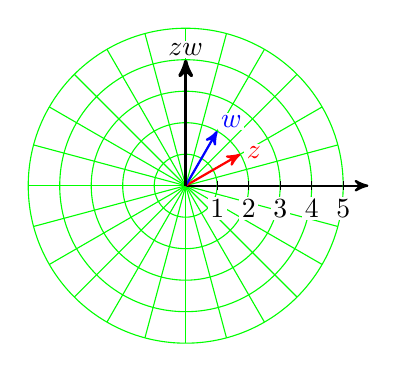
\begin{tikzpicture} [scale=.4]
\coordinate(O) at (0,0);
\foreach \angle [count=\xi] in {0, 15, ..., 345}{
  \draw[green] (\angle:0) -- (\angle:5);
}
\draw[black,thick,->,>=stealth'] (O)--(5.8,0);
\foreach \r in {1,2,3,4,5} {
\draw[green] (O) circle (\r);
\draw[black] (\r,.15) --++ (0,-.3) node[below, yshift=-2, fill=white, inner sep=1]{$\r$};
}
\coordinate (O) at (0,0);
\coordinate (z) at (30:2);
\coordinate (w) at (60:2);
\draw[red, thick, ->, >=stealth'] (O) -- (z) node[above right, xshift=1, yshift=-.1cm, fill=white, inner sep=1]{$z$};
\draw[blue, thick, ->, >=stealth'] (O) -- (w) node[above right, fill=white, inner sep=1]{$w$};
\draw[black, very thick, ->, >=stealth'] (O) -- (90:4) node[above, fill=white, inner sep=1]{$zw$};

\end{tikzpicture}
\newline



exam10-4-4

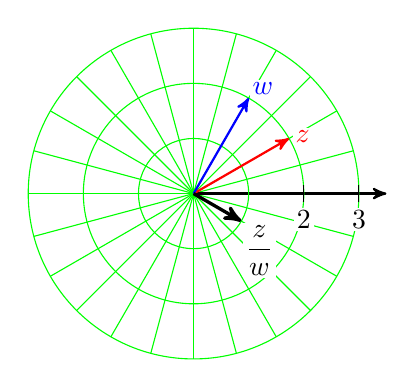
\begin{tikzpicture} [scale=.7]
\coordinate(O) at (0,0);
\foreach \angle [count=\xi] in {0, 15, ..., 345}{
  \draw[green] (\angle:0) -- (\angle:3);
}
\draw[black,thick,->,>=stealth'] (O)--(3.5,0);
\foreach \r in {2,3} {
\draw[green] (O) circle (\r);
\draw[black] (\r,.15) --++ (0,-.3) node[below, yshift=-2, fill=white, inner sep=1]{$\r$};
}
\draw[green] (O) circle (1);
\coordinate (O) at (0,0);
\coordinate (z) at (30:2);
\coordinate (w) at (60:2);
\draw[red, thick, ->, >=stealth'] (O) -- (z) node[above right, xshift=1, yshift=-.1cm, fill=white, inner sep=1]{$z$};
\draw[blue, thick, ->, >=stealth'] (O) -- (w) node[above right, fill=white, inner sep=1]{$w$};
\draw[black, very thick, ->, >=stealth'] (O) -- (-30:1) node[below right, fill=white, inner sep=1]{$\displaystyle\frac{z}{w}$};

\end{tikzpicture}
\newline



fig10-4-2

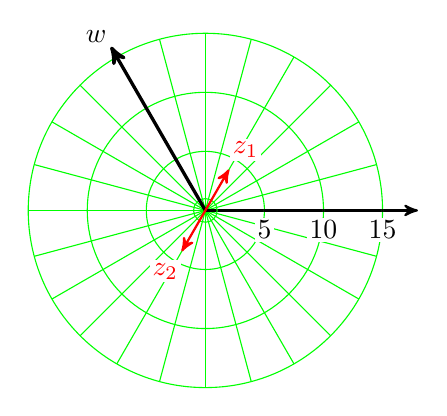
\begin{tikzpicture} [scale=.15]
\coordinate(O) at (0,0);
\foreach \angle [count=\xi] in {0, 15, ..., 345}{
  \draw[green] (\angle:0) -- (\angle:15);
}
\draw[black,thick,->,>=stealth'] (O)--(18,0);
\foreach \r in {5,10,15} {
\draw[green] (O) circle (\r);
\draw[black] (\r,.15) --++ (0,-.3) node[below, yshift=-2, fill=white, inner sep=1]{$\r$};
}
\draw[green] (O) circle (1);
\coordinate (O) at (0,0);
\coordinate (z1) at (60:4);
\coordinate (z2) at (240:4);
\coordinate (w) at (120:16);
\draw[black, very thick, ->, >=stealth'] (O) -- (w) node[above left, fill=white, inner sep=1]{$w$};
\draw[red, thick, ->, >=stealth'] (O) -- (z1) node[above right,  yshift=.1cm, fill=white, inner sep=1]{$z_1$};
\draw[red, thick, ->, >=stealth'] (O) -- (z2) node[below left, yshift=-.1cm, fill=white, inner sep=1]{$z_2$};

\end{tikzpicture}
\newline



exam10-4-6 cube roots

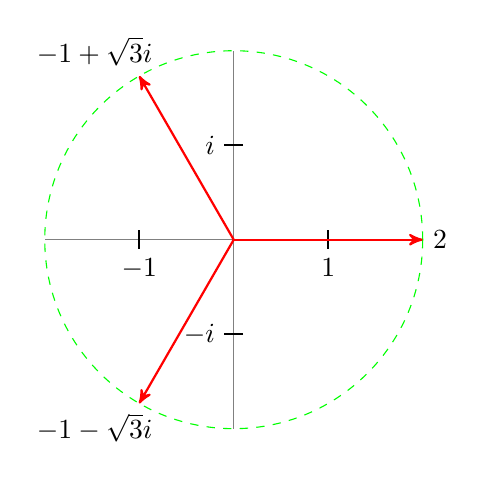
\begin{tikzpicture} [scale=1.2]
\coordinate(O) at (0,0);
\draw[gray] (-2,0) -- (O);
\draw[gray] (0,-2) -- (0,2);
\foreach \r in {1} {
\draw[black, thick] (\r,.1) --++ (0,-.2) node[below, yshift=-2, fill=white, inner sep=1]{$\r$};
\draw[black, thick] (-\r,.1) --++ (0,-.2) node[below, yshift=-2, fill=white, inner sep=1]{$-\r$};
\draw[black, thick] (.1,\r) --++ (-.2,0) node[left, xshift=-2, fill=white, inner sep=1]{$i$};
\draw[black, thick] (.1,-\r) --++ (-.2,0) node[left, xshift=-2, fill=white, inner sep=1]{$-i$};
}
\draw[green, dashed] (O) circle (2);
\coordinate (O) at (0,0);
\coordinate (z1) at (0:2);
\coordinate (z2) at (120:2);
\coordinate (z3)at (240:2);
\draw[red, thick, ->, >=stealth'] (O) -- (z1) node[right, text=black]{$2$};
\draw[red, thick, ->, >=stealth'] (O) -- (z2) node[above left, xshift=.3cm, text=black]{$-1+\sqrt{3}i$};
\draw[red,  thick, ->, >=stealth'] (O) -- (z3) node[below left, xshift=.3cm, text=black]{$-1-\sqrt{3}i$};

\end{tikzpicture}
\newline


hp10-4-1ans

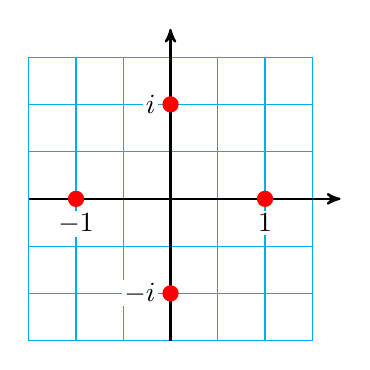
\begin{tikzpicture} [scale=1.2]
\draw[cyan] (-3/2,-3/2) grid[step=1/2] (3/2,3/2);
\draw[black,thick,->,>=stealth'] (-1.5,0)--(1.8,0);
\draw[black,thick,->,>=stealth'] (0,-1.5)--(0, 1.8);
\filldraw[red] (1,0) circle (.08cm) node[below, yshift=-.15cm, fill=white, inner sep=1, text=black]{$1$};
\filldraw[red] (0,1) circle (.08cm) node[ left, xshift=-.15cm, fill=white, inner sep=1, text=black]{$i$};
\filldraw[red] (-1,0) circle (.08cm) node[below , yshift=-.15cm, fill=white, inner sep=1, text=black]{$-1$};
\filldraw[red] ((0,-1) circle (.08cm) node[left, xshift=-.15cm, fill=white, inner sep=1, text=black]{$-i$};
\end{tikzpicture}
\newline


hp10-4-3ans

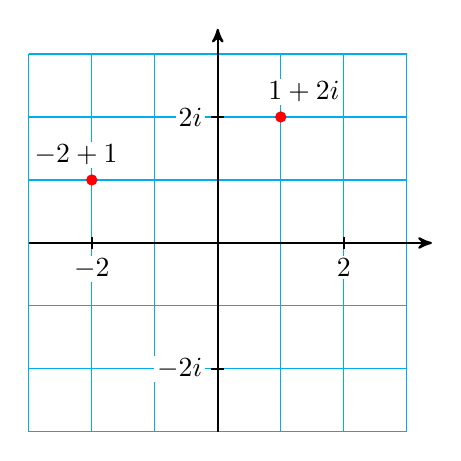
\begin{tikzpicture} [scale=0.8]
\draw[cyan] (-3,-3) grid (3,3);
\draw[black,thick,->,>=stealth'] (-3,0)--(3.4,0);
\draw[black,thick,->,>=stealth'] (0,-3)--(0, 3.4);
\foreach \r in {2} {
\draw[black, thick] (\r,.1) --++ (0,-.2) node[below, yshift=-2, fill=white, inner sep=1]{$\r$};
\draw[black, thick] (-\r,.1) --++ (0,-.2) node[below, yshift=-2, fill=white, inner sep=1]{$-\r$};
\draw[black, thick] (.1,\r) --++ (-.2,0) node[left, xshift=-2, fill=white, inner sep=1]{$\r i$};
\draw[black, thick] (.1,-\r) --++ (-.2,0) node[left, xshift=-2, fill=white, inner sep=1]{$-\r i$};
}
\filldraw[red] (1,2) circle (.08cm) node[above right, xshift=-.2cm, yshift=.15cm, fill=white, inner sep=1, text=black]{$1+2i$};
\filldraw[red] (-2,1) circle (.08cm) node[above, xshift=-.2cm, yshift=.15cm, fill=white, inner sep=1, text=black]{$-2+1$};
\end{tikzpicture}
\newline


hp10-4-43ans

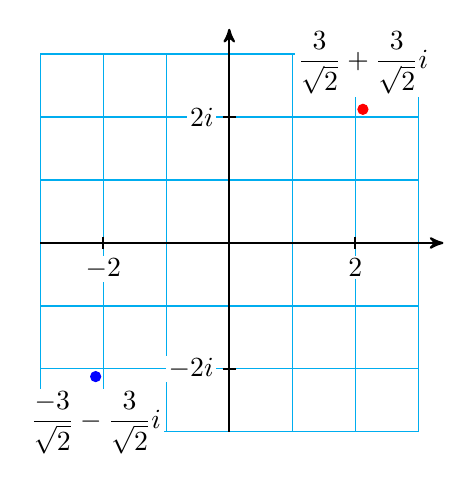
\begin{tikzpicture} [scale=0.8]
\draw[cyan] (-3,-3) grid (3,3);
\draw[black,thick,->,>=stealth'] (-3,0)--(3.4,0);
\draw[black,thick,->,>=stealth'] (0,-3)--(0, 3.4);
\foreach \r in {2} {
\draw[black, thick] (\r,.1) --++ (0,-.2) node[below, yshift=-2, fill=white, inner sep=1]{$\r$};
\draw[black, thick] (-\r,.1) --++ (0,-.2) node[below, yshift=-2, fill=white, inner sep=1]{$-\r$};
\draw[black, thick] (.1,\r) --++ (-.2,0) node[left, xshift=-2, fill=white, inner sep=1]{$\r i$};
\draw[black, thick] (.1,-\r) --++ (-.2,0) node[left, xshift=-2, fill=white, inner sep=1]{$-\r i$};
}
\filldraw[red] (45:3) circle (.08cm) node[above, yshift=.15cm, fill=white, inner sep=1, text=black]{$\displaystyle\frac{3}{\sqrt2}+\frac{3}{\sqrt2}i$};
\filldraw[blue] (225:3) circle (.08cm) node[below, yshift=-.15cm, fill=white, inner sep=1, text=black]{$\displaystyle\frac{-3}{\sqrt2}-\frac{3}{\sqrt2}i$};
\end{tikzpicture}
\newline


hp10-4-45ans

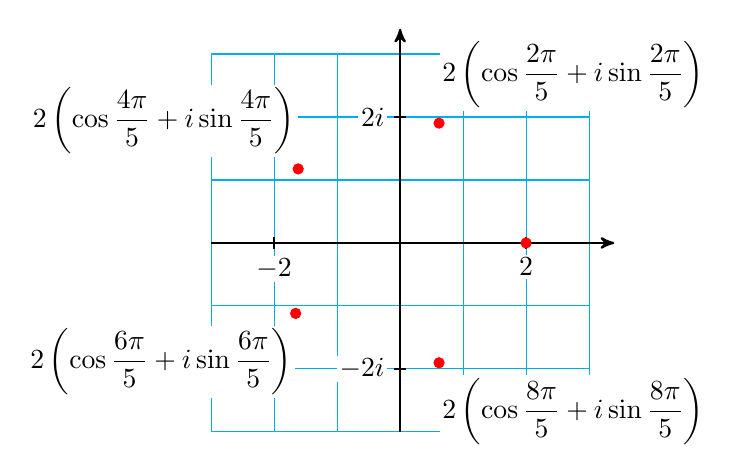
\begin{tikzpicture} [scale=0.8]
\draw[cyan] (-3,-3) grid (3,3);
\draw[black,thick,->,>=stealth'] (-3,0)--(3.4,0);
\draw[black,thick,->,>=stealth'] (0,-3)--(0, 3.4);
\foreach \r in {2} {
\draw[black, thick] (\r,.1) --++ (0,-.2) node[below, yshift=-2, fill=white, inner sep=1]{$\r$};
\draw[black, thick] (-\r,.1) --++ (0,-.2) node[below, yshift=-2, fill=white, inner sep=1]{$-\r$};
\draw[black, thick] (.1,\r) --++ (-.2,0) node[left, xshift=-2, fill=white, inner sep=1]{$\r i$};
\draw[black, thick] (.1,-\r) --++ (-.2,0) node[left, xshift=-2, fill=white, inner sep=1]{$-\r i$};
}
\filldraw[red] (0:2) circle (.08cm) node[below, yshift=-.15cm, fill=white, inner sep=1, text=black]{$2$};
\filldraw[red] (72:2) circle (.08cm) node[above right, yshift=.15cm, fill=white, inner sep=1, text=black]{$\displaystyle2\left(\cos\frac{2\pi}{5}+i\sin\frac{2\pi}{5}\right)$};
\filldraw[red] (144:2) circle (.08cm) node[above left, yshift=.15cm, fill=white, inner sep=1, text=black]{$\displaystyle2\left(\cos\frac{4\pi}{5}+i\sin\frac{4\pi}{5}\right)$};
\filldraw[red] (214:2) circle (.08cm) node[below left, yshift=-.15cm, fill=white, inner sep=1, text=black]{$\displaystyle2\left(\cos\frac{6\pi}{5}+i\sin\frac{6\pi}{5}\right)$};
\filldraw[red] (-72:2) circle (.08cm) node[below right, yshift=-.15cm, fill=white, inner sep=1, text=black]{$\displaystyle2\left(\cos\frac{8\pi}{5}+i\sin\frac{8\pi}{5}\right)$};
\end{tikzpicture}
\newline


hp10-4-47ans

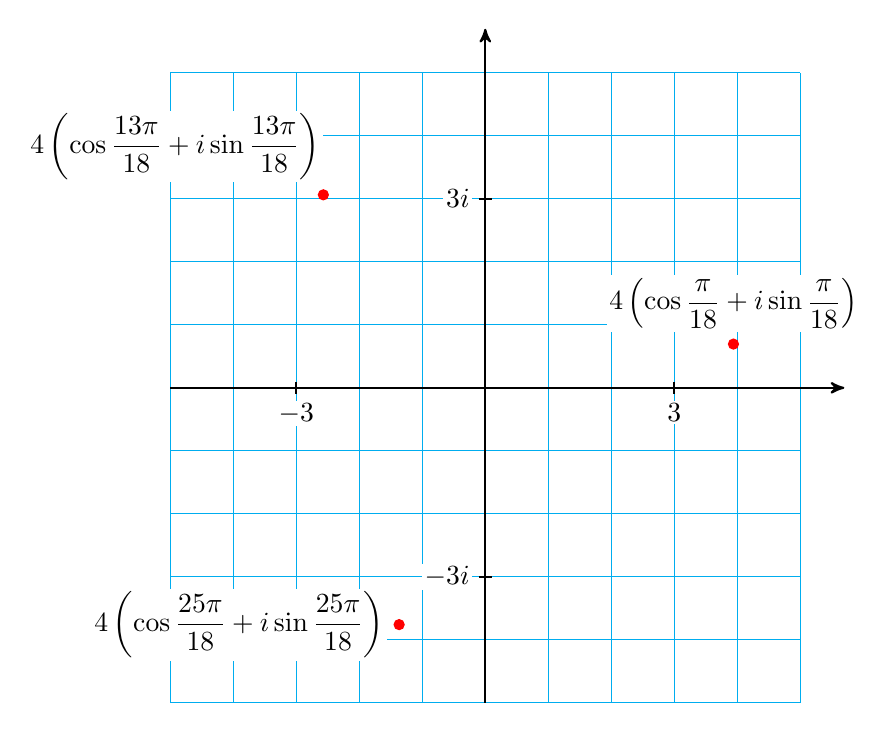
\begin{tikzpicture} [scale=0.8]
\draw[cyan] (-5,-5) grid (5,5);
\draw[black,thick,->,>=stealth'] (-5,0)--(5.7,0);
\draw[black,thick,->,>=stealth'] (0,-5)--(0, 5.7);
\foreach \r in {3} {
\draw[black, thick] (\r,.1) --++ (0,-.2) node[below, yshift=-2, fill=white, inner sep=1]{$\r$};
\draw[black, thick] (-\r,.1) --++ (0,-.2) node[below, yshift=-2, fill=white, inner sep=1]{$-\r$};
\draw[black, thick] (.1,\r) --++ (-.2,0) node[left, xshift=-2, fill=white, inner sep=1]{$\r i$};
\draw[black, thick] (.1,-\r) --++ (-.2,0) node[left, xshift=-2, fill=white, inner sep=1]{$-\r i$};
}
\filldraw[red] (10:4) circle (.08cm) node[above, yshift=.15cm, fill=white, inner sep=1, text=black]{$\displaystyle 4\left(\cos\frac{\pi}{18}+i\sin\frac{\pi}{18}\right)$};
\filldraw[red] (130:4) circle (.08cm) node[above left, yshift=.15cm, fill=white, inner sep=1, text=black]{$\displaystyle 4\left(\cos\frac{13\pi}{18}+i\sin\frac{13\pi}{18}\right)$};
\filldraw[red] (250:4) circle (.08cm) node[ left, xshift=-.15cm, fill=white, inner sep=1, text=black]{$\displaystyle 4\left(\cos\frac{25\pi}{18}+i\sin\frac{25\pi}{18}\right)$};
\end{tikzpicture}
\newline



hp10-1-1 polar grid

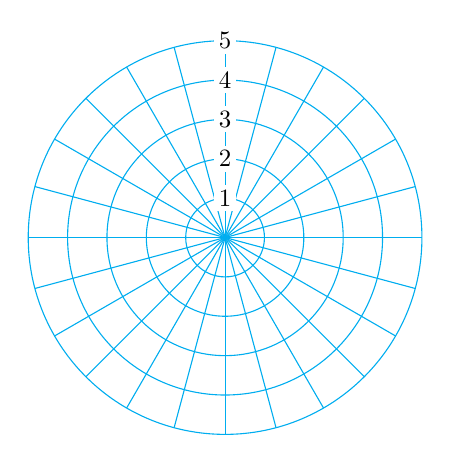
\begin{tikzpicture} [scale=.5]
\coordinate(O) at (0,0);
\foreach \angle [count=\xi] in {0, 15, ..., 345}{
  \draw[cyan] (\angle:0) -- (\angle:5);
}
\foreach \r in {1,2,3,4,5} {
\draw[cyan] (O) circle (\r);
\node[fill=white, inner sep = 2, text=black, scale=.9] at (90:\r) {$\r$};
}

\end{tikzpicture}
\newline


hp10-rev-1ans polar plot

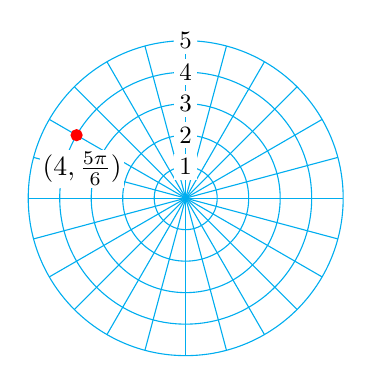
\begin{tikzpicture} [scale=.4]
\coordinate(O) at (0,0);
\foreach \angle [count=\xi] in {0, 15, ..., 345}{
  \draw[cyan] (\angle:0) -- (\angle:5);
}
\foreach \r in {1,2,3,4,5} {
\draw[cyan] (O) circle (\r);
\node[fill=white, inner sep = 2, text=black, scale=.9] at (90:\r) {$\r$};
}
\filldraw[red] (150:4) circle (5pt) node[below, xshift=2, yshift=-5, text=black, fill=white, inner sep=1]{$(4,\frac{5\pi}{6})$};
\end{tikzpicture}
\newline


hp10-rev-3ans polar plot

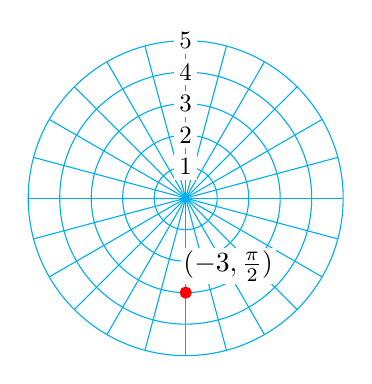
\begin{tikzpicture} [scale=.4]
\coordinate(O) at (0,0);
\foreach \angle [count=\xi] in {0, 15, ..., 345}{
  \draw[cyan] (\angle:0) -- (\angle:5);
}
\foreach \r in {1,2,3,4,5} {
\draw[cyan] (O) circle (\r);
\node[fill=white, inner sep = 2, text=black, scale=.9] at (90:\r) {$\r$};
}
\filldraw[red] (90:-3) circle (5pt) node[above right, xshift=-2, yshift=3, text=black, fill=white, inner sep=1]{$(-3,\frac{\pi}{2})$};
\end{tikzpicture}
\newline


hp10-rev-13ans polar plot


\begin{tikzpicture} [scale=.5]
\coordinate(O) at (0,0);
\path [draw=none,fill=yellow, fill opacity = 0.6] (O)--(-45:5) arc (45:5) -- (O);
\draw[cyan, thick] (-45:5)--(O)--(45:5);


\foreach \angle [count=\xi] in {0, 15, ..., 345}{
  \draw[cyan] (\angle:0) -- (\angle:5);
}
\foreach \r in {1,2,3,4,5} {
\draw[cyan] (O) circle (\r);
\node[fill=white, inner sep = 2, text=black, scale=.9] at (90:\r) {$\r$};
}

\end{tikzpicture}
\newline






\end{document}
